\section{Objects in the amber.crawler package}



\classname{RSS}

\begin{classmetadata}
  \extends{amber.CrawlerObject}
  \implements{amber.common.AirBrushCallable}
\end{classmetadata}

\begin{interface}
  \init{RSS}{}
    {Creates a new RSS crawler. It will wait for instructions via Psyclone,
      like which RSS feed has to be monitored.}
  \init{RSS}{URL feedurl}
    {Creates a new RSS crawler, initialized with the URL of the feed to be
      monitored.}
  \method{void}{airBrushReceiveMessage}{Message msg}
    {Callback function for AirBrushCallable.}
  \method{void}{run}{}
    {Callback function for Runnable.}
  % \method{Boolean}{addFeed}{URL}
  % {Adds a feed to the crawler. Will be crawled during the next cycle. Returns
  % true if succesful, false otherwise.}
  % \method{Boolean}{removeFeed}{}{FIXME: do or don't?}
\end{interface}



\begin{figure}
  \centering
  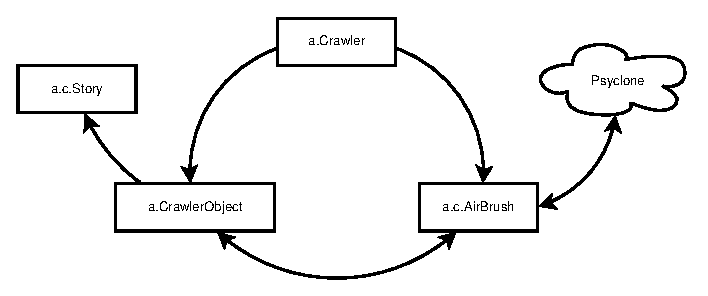
\includegraphics{image/crawler}
  \caption{
    Diagram of the design of the Crawler, the names are Java classnames
  }
\end{figure}

